% $Id: diss.tex,v 1.54 2008/05/12 14:28:09 Moritz.Ringler Exp $
% Das Latex-Paket lm muss DEINSTALLIERT werden. Sonst ersetzt
% pdflatex die opentype-Schrift in den Grafiken durch die type1-Schrift,
% was dann fehlende Glyphen zur Folge hat. Falls MikTeX versucht,
% das lm-Paket herunterzuladen und zu installieren, muss die automatische
% Paketinstallation "On-the-fly" abgeschaltet werden.
\documentclass[ %
    twoside,    % rechte und linke Seiten
    headinclude=true,
    footinclude=true,
    pointlessnumbers,
    openright      % Kapitel darf nur auf rechter Seite starten
    %bibtotoc,   % Literaturverzeichnis in das Inhaltsverzeichnis
    %liststotoc % andere Verzeichnisse aufnehmen
    %idxtotoc    % und auch den Index
]{scrartcl}
\KOMAoptions{fontsize=10pt}
\KOMAoptions{paper=a4}
\KOMAoptions{bookmarkpackage=false}
%\AtBeginDocument{\overfullrule=5pt}
\usepackage{ifthen}             % Kontroll-Strukturen

\newboolean{usehyperref}
\setboolean{usehyperref}{true} % Ausgabe von PDFs mit (true) oder ohne (false)
                               % Hyperlinks. HIER �NDERN.
\newboolean{printrcs}
\setboolean{printrcs}{false}     % Ausgabe mit (true) oder ohne (false) RCS-Versionsinformation

\newcommand{\disstitle}{GMM-FIELD and GMM-DIP}

% Ab hier nichts aendern.
\ifpdfoutput{}{\setboolean{usehyperref}{false}} % Hyperref nur bei pdf-Ausgabe
\newcommand{\ifhyperref}[2]{
    \ifthenelse{\boolean{usehyperref}}{#1}{#2}} % hyperref ja oder nein

\newcommand{\ifrcs}[2]{
    \ifthenelse{\boolean{printrcs}}{#1}{#2}} % pritnrcs ja oder nein
% alles was man fuer Formeln braucht...
\usepackage[
    fleqn          % Glgen nicht zentriert, sondern mit fester Einr�ckung.
]{
    amsmath        % AMS Mathematik-Paket
}
\usepackage{                    % alles was man fuer Formeln braucht...
    amssymb,                    % AMS mathematische Symbole
    amsfonts,                   % AMS Schriftarten
    fixmath,                    % kursive griechische Grossbuchstaben im Mathematikmodus
    icomma                      % Komma als Dezimaltrennzeichen im
                                % Mathematikmodus (ausser wenn vor Leerzeichen)
}
\usepackage{pxfonts}            % Schriftart Palatino
\renewcommand{\sfdefault}{cmss} % Computer Modern als Groteskschrift
% Wuerde hier gerne Latin Modern verwenden. Das geht aber nicht, weil pdflatex
% dann versucht den von Illustrator aus der OpenType-Version erzeugten
% Latin Modern Type 1C Font in den Grafiken durch den Type 1 Font des
% TeX-Systems zu substituieren und dabei ueber fehlende Glyphen stolpert,
% die sich dann als Luecken im Grafiktext
% auswirken. Das alles, wenn Latin Modern auch nur im
% TeX System *installiert* ist.
% Vermutlich kann man das verhindern, indem man irgendeine <font>.map Datei
% editiert. Stattdessen habe ich jetzt einfach das lm-Paket komplett
% deinstalliert.

\usepackage{setspace}
\AtBeginDocument{\onehalfspacing}

\usepackage[a4paper]{geometry}   % Besseres Seitenlayout als mit KOMA
\usepackage[automark]{scrpage2}  % scrpage
\usepackage{setspace}            % Doppelter Zeilenabstand auf Titelseite

\usepackage[                    % ein Symbol-Verzeichnis
    german,                     % auf Deutsch
    refpage,                    % mit Seitenzahl der ersten Verwendung
    notintoc                    % nicht im Inhaltsverzeichnis
]{nomencl}
\renewcommand{\nompreamble}{Zahlenwerte fuer physikalische Konstanten nach
CODATA \cite{CODATA2006}.}
\usepackage{index}              % Indices, muss VOR hyperref eingebunden werden

\ifhyperref{
  \usepackage[              % Hyperlinks...
      hyperfootnotes=false, % keine verlinkten Fu�noten
      hyperindex=true,      % verlinkter Index
      %pagebackref=true,     % R�ckreferenzen aus dem Literaturverzeichnis
      bookmarks=true,       % Erzeuge pdf bookmarks
      colorlinks = false,   % Keine farbige Linkauszeichnung
      pdfborder=0 0 0,      % Keine Boxen um Links
      breaklinks=true,
      pdftitle={\disstitle},
      pdfauthor={Moritz Ringler},
      pdfcreator={Moritz Ringler},
      pdfpagelayout=TwoPageRight, % doppelseitig mit ungerade Seiten rechts
                                  % nicht-fortlaufende Anzeige
      pdfstartview=Fit,           % ganze Seite an Fenster anpassen
      pdflang=DE
  ]{hyperref}
}{% wenn keine Hyperrefs
    \usepackage[pageref]{backref} % trotzdem Rueckverweise
}
\ifthenelse{\isundefined{\href}}{
    \newcommand{\href}[2]{#2}     % nur Anker ausgeben
                                  % Diese Definiton wird benoetigt, um
                                  % den mit url-bst erstellten
                                  % Bibliographiestil auch ohne
                                  % Hyperref nutzen zu koennen
}{}

%\usepackage{a4}            % benutzt DIN A4 Papierformat
%\usepackage[english, ngerman]{babel}      % deutsch nach neuer RS
\usepackage[                    % schlauere Zitate
    numbers,
    sort&compress
]{
    natbib
}
\ifhyperref{
    \usepackage{hypernat}  % hyperref Erweiterungen zu natbib
}{}

    \usepackage{microtype} % pdftex microtypographic features
                           % -> weniger Box-Probleme

\usepackage{
    graphicx,                   % Grafikeinbindung
    color,                      % Farbe
    rcs                         % RCS-Versionsinformationen
}

\usepackage[perpage]{footmisc}  % Fussnoten pro Seite nummerieren
\usepackage{
    soul                        % Letterspacing, Kapitaelchen
}
\usepackage[latin1]{inputenc}   % ISO-8859-1 kodierter Text
\usepackage[T1]{fontenc}        % T1-kodierte Schrift
\usepackage{
    textcomp,                   % Symbole im Text (needed for gensymb)
    gensymb                     % generische Symbole und aufrechtes \mu
}
\usepackage[                    % Bild- und Tabellenbeschriftungen
    format = plain,
    font=footnotesize,
    labelfont=bf
]{caption}
\usepackage{sidecap}            % Captions auch neben dem Bild.

\usepackage{tocvsec2}           % Erlaubt lokales Setzen der Tiefe des TOCs
                                % via \settocdepth

\usepackage[figure]{algorithm2e} % Pseudocode. Das Paket erzeugt
                                 % allerdings bei jedem Algorithmus seltsame
                                 % hbox-Warnungen. Naja, zu spaet, das noch zu
                                 % aendern.

\usepackage{color}

\usepackage{microtype} %

%\clubpenalty=10000
%\widowpenalty=10000
%\displaywidowpenalty=10000
           % Seitenumbruchkontrolle. Keine Ahnung ob's funktioniert...

%% global definitions
% $Id: definitionen.tex,v 1.33 2008/03/11 09:02:38 Moritz.Ringler Exp $

% Layout und Satz
%---------------------------------------------
%Kopf- und Fusszeile
\pagestyle{scrheadings}
\clearscrheadings
\clearscrplain
\lohead{\headmark}
\ifrcs{
    \lofoot{\RCSId}
    \refoot{\RCSId}
}{}
\lefoot[\pagemark]{\pagemark}
\rofoot[\pagemark]{\pagemark}
\setfootsepline{.4pt} % Ganzunten
%---------------------------------------------
% Rueckverweise im Literaturverzeichnis
%\renewcommand*{\backref}[1]{} % backref wird ausgeschaltet
%\renewcommand*{\backrefalt}[4]{ % backrefalt umdefiniert
%\ifcase #1 %keine Seite
%[nicht zitiert] %
%\or % genau eine Seite
%\mbox{[$\rightarrow$ Seite #2]}
%\else % mehrere Seiten
%\mbox{[$\rightarrow$ Seiten #2]}
%\fi
%}
% Zeichenkette zwischen genau 2 Seiten
%\renewcommand*{\backreftwosep}{ und~}
% Zeichenkette zwischen den beiden letzten von > 2 Seiten
%\renewcommand*{\backreflastsep}{ und~}
%----------------------------------------------
% Captions
%\renewcommand{\captionlabelsep}{\/\ }
%----------------------------------------------
% Sonstige Verzeichnisse, Indices
% Symbolverzeichnis


%Standardindex
% default: Dies ist der Standardindex, es muss kein Bezeichner angegeben werden
% idx: Erweiterung fuer MakeIndex-Eingabedatei
% ind: Erweiterung fuer MakeIndex-Ausgabedatei
% Index: Name fuer den Index
\newindex{default}{idx}{ind}{Index}

%\sloppy

\newcommand{\uri}[1]{\href{#1}{#1}}

\newenvironment{myTitlepage}{ %
    \thispagestyle{empty}
    \addtolength{\oddsidemargin}{0.5cm}
    \begin{titlepage}
    %\addtolength{\textwidth}{1.6cm}
    \begin{minipage}{\textwidth}
    \centering
}{
    \end{minipage}
    %\addtolength{\textwidth}{-1.6cm}
    \enlargethispage{5 \baselineskip}
    \end{titlepage}
    \addtolength{\oddsidemargin}{0.5cm}
}
%\numberwithin{equation}{section}

%\renewcommand{\baselinestretch}{1.5}
\renewcommand{\arraystretch}{0.97}
\newcommand{\foreign}[1]{\textsl{#1}}
\newcommand{\begriff}[1]{{#1}}
\newcommand{\refeqn}[1]{Eq.~\eqref{#1}}
%thesis class benutzt fuer captions \figureshortname,
%wird in ngerman.sty/german.sty nicht umdefiniert.
%\newcommand{\figureshortname}{Abb.}
\newcommand{\reffig}[1]{Fig.~\ref{#1}}
\newcommand{\refsec}[1]{Sec.~\ref{#1}}
%\newcommand{\refapp}[1]{Anhang~\ref{#1}}
%\newcommand{\reftab}[1]{Tabelle~\ref{#1}}
\newcommand{\code}[1]{{\texttt{#1}}}
\newcommand{\bookmark}[3][]{\ifhyperref{\hypertarget{#3}{}\pdfbookmark[#1]{#2}{#3}}{}}
\renewcommand{\dictumwidth}{0.41 \textwidth}

% Meta-Daten
% uncomment exactly one of the following two lines
%\newcommand{\cvsvers}{}
\newcommand{\cvsvers}{{\tiny(Rev. \RCSRevision{}, \RCSDate{})\newline}}

% numerische Werte
\newcommand{\eee}[1]{\ensuremath{10^{#1}}}
\newcommand{\val}[2]{\ensuremath{#1}\text{\,#2}}
\newcommand{\ee}[2]{\ensuremath{#1\times\eee{#2}}}
\newcommand{\valee}[3]{\val{\ee{#1}{#2}}{#3}}
\newcommand{\mikro}[1]{\ensuremath{\text{\micro#1}}}
\newcommand{\ftow}[1]{\ensuremath{2\pi \!\times\!#1}}

% nanoantenna.tex
\newcommand{\wexc}{\ensuremath{\omega_\mathrm{exc}}}
\newcommand{\rexc}{\ensuremath{\gamma_\mathrm{exc}}}
\newcommand{\rexci}{\ensuremath{\gamma_{\mathrm{exc}\, 0}}}
\newcommand{\qe}{\ensuremath{\eta}}
\newcommand{\rr}{\ensuremath{\gamma_\mathrm{r}}}
\newcommand{\rri}{\ensuremath{\gamma_{\mathrm{r}\, 0}}}
\newcommand{\ret}{\ensuremath{\gamma_\mathrm{ET}}}
\newcommand{\rfluo}{\ensuremath{\gamma_\mathrm{Fluo}}}
\newcommand{\rxr}{\ensuremath{\gamma_{\mathrm{nr}}}}

% chem. Elemente
\newcommand{\element}[2]{#1 #2}
\newcommand{\selement}[2]{\ensuremath{\kern0.05em^{#2}}\kern-0.1em#1}

% thermodyn. und statistische Groessen
\newcommand{\ldb}{\ensuremath{\lambda_{\mathrm{dB}}}}
\newcommand{\kb}{\ensuremath{k_\mathrm{B}}}
\newcommand{\visc}{\ensuremath{\tilde{\eta}}}
%\newcommand{\Tkrit}{\ensuremath{T_c}}
%\newcommand{\Tdop}{\ensuremath{T\!_\mathrm{D}}}
%\newcommand{\dm}{\qop{\rho}}
%\newcommand{\dmel}[2]{\ensuremath{ \rho_{#1 #2}}}

%Goldpartikel
\newcommand{\npr}{\ensuremath{R}} %Nanopartikelradius
\newcommand{\cro}[1]{\ensuremath{\sigma_{\mathrm{#1}}}} % Wirkungsquerschnitt

%dielektr. Funktion
\newcommand{\epsi}[1]{\ensuremath{\varepsilon_{\mathrm{#1}}}}
\newcommand{\epsint}{\epsi{\mathcal{I}}}
\newcommand{\epsext}{\epsi{\mathcal{A}}}

% mathematische Konstrukte
% a function named #1 with argument #2; both in math
\newcommand{\func}[2]{\ensuremath{#1 \text{\small$\left(#2\right)$}}}

\renewcommand{\vec}[2][]{\ensuremath{\boldsymbol{#2}_{#1}}}
\renewcommand{\Re}{\mathfrak{Re}\kern-0.05em}
\renewcommand{\Im}{\mathfrak{Im}}

% Einheitsvektoren
\newcommand{\er}{\ensuremath{\vec[r]{\hat{e}}}}
\newcommand{\ex}{\ensuremath{\vec[x]{\hat{e}}}}
\newcommand{\ephi}{\ensuremath{\vec[\phi]{\hat{e}}}}
\newcommand{\etheta}{\ensuremath{\vec[\theta]{\hat{e}}}}

% em Felder und andere vektorielle Groessen

\newcommand{\evec}{\ensuremath{\vec{E}}}
\newcommand{\hvec}{\ensuremath{\vec{H}}}
\newcommand{\kvec}{\ensuremath{\vec{k}}}
\newcommand{\eovec}{\ensuremath{\vec[0]{E}}}
\newcommand{\escat}{\ensuremath{\vec[\mathrm{str}]{E}}}
\newcommand{\eint}{\ensuremath{\vec[\mathcal{I}]{E}}}
\newcommand{\einc}{\ensuremath{\vec[\mathrm{in}]{E}}}
\newcommand{\hscat}{\ensuremath{\vec[\mathrm{str}]{H}}}
\newcommand{\hint}{\ensuremath{\vec[\mathcal{I}]{H}}}
\newcommand{\hinc}{\ensuremath{\vec[\mathrm{in}]{H}}}
\newcommand{\bvec}{\ensuremath{\vec{B}}}
\newcommand{\rvec}{\ensuremath{\vec{r}}}
\newcommand{\rovec}{\ensuremath{\vec[0]{r}}}
\newcommand{\evecr}{\func{\evec}{\rvec}}
\newcommand{\hvecr}{\func{\hvec}{\rvec}}
\newcommand{\pvec}{\ensuremath{\vec{S}}}
\newcommand{\pvect}[1]{\ensuremath{\vec[\mathrm{#1}]{S}}}

% Mietheorie
\newcommand{\mmnj}{\ensuremath{\boldsymbol{M}^j_{mn}}}
\newcommand{\nmnj}{\ensuremath{\boldsymbol{N}^j_{mn}}}
\newcommand{\mmnbj}{\ensuremath{\boldsymbol{M}^{j\;\beta}_{mn}}}
\newcommand{\nmnbj}{\ensuremath{\boldsymbol{N}^{j\;\beta}_{mn}}}
\newcommand{\mm}[2]{\ensuremath{\boldsymbol{M}^{\,#1\, #2}_{mn}}}
\newcommand{\nn}[2]{\ensuremath{\boldsymbol{N}^{\,#1\, #2}_{mn}}}

\newcommand{\mmn}[1]{\ensuremath{\boldsymbol{M}^{#1}_{mn}}}
\newcommand{\nmn}[1]{\ensuremath{\boldsymbol{N}^{#1}_{mn}}}
\newcommand{\pimn}{\ensuremath{\pi_{mn}}}
\newcommand{\taumn}{\ensuremath{\tau_{mn}}}
\newcommand{\pmn}{\ensuremath{P^m_n}}
\newcommand{\emn}{\ensuremath{E_{mn}}}
\newcommand{\reln}{\ensuremath{\nu}}
\newcommand{\tilmn}{\ensuremath{{\tilde{m}\tilde{n}}}}

\newcommand{\lmax}{\ensuremath{\lambda_\mathrm{max}}}

\newcommand{\rvecp}[1][]{\ensuremath{\rvec{#1}'}}
\newcommand{\ri}[1]{\ensuremath{r_{#1}}}
\newcommand{\ucv}[1]{\ensuremath{\vec[#1]{e}}}
\newcommand{\magdip}{p}
%\newcommand{\xioffe}{x\kern-0.1em_I}
%\newcommand{\yioffe}{y\kern-0.1em_I}
%\newcommand{\zioffe}{z\kern-0.1em_I}


% the scalar product of #1 and #2
\newcommand{\scp}[2]{\ensuremath{#1 \cdot #2}}
% complex conjugate
\newcommand{\conj}[1]{\ensuremath{#1^{*}}}
% imaginary i
\newcommand{\imi}{\ensuremath{i}}
% upright d for integrals
\newcommand{\dint}{\text{d}}
% derivative d#1/d#2
\newcommand{\deriv}[2]{\ensuremath{\frac{\mathrm{d}#1}{\mathrm{d}#2}}}
\newcommand{\diff}[1]{\ensuremath{\frac{\mathrm{d}}{\mathrm{d}#1}}}
% exponential function as e^#1
\newcommand{\expe}[1]{\ensuremath{\text{e}^{#1}}}
% exponential function as exp(#1)
\renewcommand{\exp}[1]{\func{\text{exp}}{#1}}
% the big O for approximations
\newcommand{\bigo}[1]{\ensuremath{\func{\mathcal{O}}{#1}}}
% constant
\newcommand{\const}{\ensuremath{const}}
% the dirac delta "function"
\newcommand{\dirac}[1][\rvec]{\ensuremath{\func{\delta}{#1}}}
% a statistical average < #1 >
\newcommand{\statav}[1]{\langle #1\rangle}
% an equals sign with not too much space around it
\newcommand{\teq}{\kern-0.27em=\kern-0.1em} % tight equals
% the absolute value of something
\newcommand{\abs}[1]{\lvert#1\rvert}
% the vector norm
\newcommand{\vnorm}[1]{\ensuremath{\|#1\|}}
% the laplace operator
\newcommand{\lapl}{\triangle}
% the nabla operator
%\newcommand{\nabla}{\triangledown}
% the divergence operator
\DeclareMathOperator{\divergence}{div}

% QM
% dirac notation bra, ket, bracket, matrix element
\newcommand{\bra}[1]{\mbox{\ensuremath{\langle #1|}}}
\newcommand{\ket}[1]{\mbox{\ensuremath{| #1\rangle}}}
\newcommand{\braket}[2]{\mbox{\ensuremath{\langle #1| #2\rangle}}}
\newcommand{\mel}[3]{\ensuremath{\langle #2|#1| #3\rangle}}
% a function operator
\newcommand{\fop}[1][\rvec]{\widehat{\Psi}\text{\footnotesize$(#1, t)$}}
\newcommand{\fopi}[1]{\widehat{\Psi#1}\text{\footnotesize$(\rvec, t)$}}
\newcommand{\fopc}[1][\rvec]{\widehat{\Psi}^+\!\text{\footnotesize$(#1, t)$}}
% any quantum mechanical operator
\newcommand{\qop}[1]{\ensuremath{\widehat{#1}}}
% the bohr magneton
\newcommand{\mubohr}{\mu\kern-0.07em_\mathrm{B}}
\newcommand{\wf}[1][]{\ensuremath{\phi_\mathrm{#1}}}
\newcommand{\qnorm}[1]{\|#1\|_{\mathcal{L}^2}}


\newcommand{\konz}{\ensuremath{c_\mathrm{mol}}}
\newcommand{\csq}{\ensuremath{\chi^2}}

%Sonstige
\newcommand{\incflux}{\ensuremath{S_\mathrm{in}}}
\newcommand{\excflux}{\ensuremath{S_\mathrm{exc}}}
\newcommand{\dss}{\ensuremath{\tilde{d}}}
\newcommand{\registered}{\text{\textregistered}}
\newcommand{\gexc}{\ensuremath{g_{\mathrm{exc}}(\omega_\mathrm{exc})}}
\newcommand{\gem}{\ensuremath{g_\mathrm{em}(\omega)}}
\newcommand{\graman}{\ensuremath{g_\mathrm{EM}}}
\newcommand{\dip}{\ensuremath{\vec{p}}}
\newcommand{\rrD}{\ensuremath{\Gamma_\mathrm{r}}}
\newcommand{\rriD}{\ensuremath{\Gamma_{\mathrm{r}\, 0}}}
\newcommand{\retD}{\ensuremath{\Gamma_\mathrm{ET}}}
\newcommand{\rnr}{\ensuremath{\gamma_{\mathrm{nr}\,0}}}
%\newcommand{\mmu}[2]{\bvec{M}_{\mu\nu}^{#1\, #2}}
%\newcommand{\nnu}[2]{\bvec{N}_{\mu\nu}^{#1\, #2}}
%\newcommand{\ajmn}{a_{mn}^j}
%\newcommand{\bjmn}{b_{mn}^j}
%\newcommand{\pjlmn}{p_{mn}^{l}}
%\newcommand{\qjlmn}{q_{mn}^{l}}
\newcommand{\grw}{\ensuremath{g_\mathrm{r}(\omega)}}
\newcommand{\getw}{\ensuremath{g_\mathrm{ET}(\omega)}}
%\newcommand{\micro}{\ensuremath{\mu}}


%% Metadata
\author{Moritz Ringler}
%\RCS $Date: 2008/05/12 14:28:09 $ \RCS $Revision: 1.54 $
%\RCS $Id: diss.tex,v 1.54 2008/05/12 14:28:09 Moritz.Ringler Exp $
\title{\disstitle}
%\subtitle{Rev. \RCSRevision, \RCSDate}
\date{July 2009}

\begin{document}
%\href{http://nbn-resolving.de/urn:nbn:de:bvb:19-84894}{urn:nbn:de:bvb:19-84894}
\numberwithin{equation}{section}
\numberwithin{figure}{section}
\numberwithin{table}{section}

% $Id: prog.tex,v 1.5 2008/02/11 19:23:22 Moritz.Ringler Exp $
% Kein unabhaengiges LaTeX-Dokument!
% Master-Dokument: diss.tex
%
\definecolor{darkblue}{rgb}{0,0.08,0.45}
\maketitle

\section{About this document}
GMM-FIELD is a computer program that calculates the local electric field in an
aggregate of spherical particles that is hit by a plane light wave. Its companion
GMM-DIP calculates the absorbed and emitted power when a Hertzian dipole is placed
inside such an aggregate. Both programs were developed as part of my PhD thesis
\cite{phdrin08}, and I used them to calculate the theoretical results published in
\cite{bek07} and \cite{rin08}. This was possible only because Yu-Lin Xu
had published the source code of GMM and because Thomas Wriedt had kept it publicly
accessible on his Electromagnetic Scattering Programs web site \cite{wwwwriedt}.
Therefore, I decided to also publish the source code of GMM-FIELD and GMM-DIP
on the web.
Thomas Wriedt soon found out and included GMM-DIP and GMM-FIELD in his list of
scattering programs. Subsequently, he was asked about an English document that
describes how the programs can be used and he forwarded this
request to me. Lacking the time to write a comprehensive manual I agreed to
translate the relevant sections of my PhD thesis, and the result is the present
document. Please also read the GMM manual included in the original GMM package,
which is hosted on the Two Particle Scattering subpage of \cite{wwwwriedt}.
If you need further assistance using GMM-FIELD and GMM-DIP feel free to contact
me at gmm@momail.e4ward.com

\section{Bugs and fixes}
The original GMM-Field and GMM-DIP used a wrong normalization for the vector
spherical wave functions. This bug was discovered and fixed by Matthew Arnold, from UTS
Sidney, Australia. The fix has been included in the web release on 2009-07-13.
The bug does not affect the cross sections (GMM-FIELD) and rates (GMM-DIP) but will lead
to wrong results for the near field. In the cases that I have tested the
results with the bug are not far off from the correct ones. But there might be
cases where they are.

On 2014-01-16, another bug was found that might lead to incorrect higher-order
contributions to the near-field when the actual truncation order nmax(i) for one
of the other spheres/particles is greater than that of the first sphere/particle.
This bug was fixed in the web release on 2014-01-16.

GMM-FIELD and GMM-DIP are based on the 2001 GMM distribution and do
not contain any fixes from the 2003 version.

\section{Citing GMM-FIELD and GMM-DIP}
If you want to cite GMM-FIELD or GMM-DIP in a scientific article I would suggest
that you cite either \cite{phdrin08} or \cite{rin08}. Please also consider citing
Yu-Lin Xu's articles on the subject \cite{xuy95, xuy95err, xuy97, xuy98}. If you
want to tell your readers where to get the code I would suggest that you refer
them to the "Two particle scattering" subsection of \cite{wwwwriedt}.

% $Id: gmmf.tex,v 1.26 2008/05/04 10:37:19 Moritz.Ringler Exp $ 
% Kein unabhaengiges LaTeX-Dokument! 
% Master-Dokument: diss.tex  
%
\section{GMM -- a Generalized Mie Scattering code}\label{app.gmmf}

The program GMM \cite{gmm01f} by Yu-Lin Xu implements Generalized Mie Scattering
according to \cite{xuy95, xuy95err, xuy97, xuy98}. The main difference from
the treatment in these articles is the use of another normalization constant $\emn$. Details
about this and a general introduction to GMM can be found in the original GMM
documentation distributed together with GMM.

For a given aggregate of spherical nanoparticles, GMM\index{GMM} calculates the
scattering, extinction and absorption cross sections\footnote{GMM also 
calculates the scattering matrix, but this is of no importance in the context
of GMM-DIP and GMM-FIELD.} for an incoming plane wave of a given wavelength.
The overall program flow is represented in figure~\ref{abb.gmm}.

\begin{algorithm}[h]
\KwData{$n_\mathrm{max}$, $\lambda$, $N$; $\vec{r}^\beta$, $R^\beta$, $\epsint^\beta$}
\KwResult{\cro{str}, \cro{ext}, \cro{abs}}
\Begin{
read wavelength\;
read aggregate parameters\;
calculate Mie coefficients for all spheres\;
calculate vector translation coefficients\;
expand the incoming wave in vector spherical harmonics $\rightarrow p_{mn}^{0\;\beta}, q_{mn}^{0\;\beta}$\;
calculate scattering coefficients for all spheres $\beta$ $\rightarrow a_{mn}^\beta, b_{mn}^\beta$\;
calculate scattering cross section\;
calculate extinction and absorption cross sections\;
output\;
}
\caption{Program flow of GMM}\label{abb.gmm}
\end{algorithm}

GMM has no external dependencies and can be compiled with the FORTRAN compilers
of the GNU Compiler Collection,
%\footnote{\uri{http://gcc.gnu.org/}}%
gfortran and g77, on all platforms where these are available. 
For \cite{phdrin08}, I used gfortran (gcc~4.2.1) under SUSE Linux and
g77 (gcc~3.4.4) under Windows/Cygwin.
%\footnote{\uri{http://cygwin.com}}. 
GMM and the commercial MQAggregates \cite{qui93}
will produce identical results when given the same input.
GMM is usually faster and easier to control from the shell,
which makes it possible to write shell scripts that
automatically calculate a series of scattering spetra e. g. for
different particle distances in a dimer.

\clearpage{}
\ifhyperref{\phantomsection}{}
\section{GMM-FIELD -- a GMM Extension that Calculates the Near Field}\index{GMM-FIELD}
To understand nanoparticle dimer resonators and to calculate fluorescence and
Raman scattering in their interior, as in \cite{rin08}, one must know the
local electric field. The original GMM calculates only far field quantities,
but it can be extended in such a way that the near field is also obtained.
GMM-FIELD is such an extension.
%
\footnote{The source code of GMM-FIELD  as well as some example applications
can be downloaded from
\mbox{\uri{http://moritz-ringler.name/dissertation/GMM\_FIELD.tar.bz2}}.}

The local field in the space 
$\mathcal{A}$ outside the particles is given by the sum
$\evec = \einc + \escat$. 
The incident field \einc{} is trivially calculated for a plane wave
as $\exp{i k z}\;\ex$. The scattered field $\escat$ can be calculated with
either of two approaches: you can expand the 
scattered field of all spheres in the vector spherical harmonics of one 
particular sphere (or another point in space) and evaluate this expansion
for all the points of the grid $G$ on which you want to know the field.
Alternatively, you can transform the cartesian coordinates of each grid point 
into the spherical coordinate systems of each sphere $\beta$, 
calculate the partial 
scattered fields $\escat^\beta$ in those coordinate systems,
and finally sum them in the original cartesian coordinate system.
I have chosen this latter approach for GMM-FIELD.
The algorithm of the routine that has been added to 
GMM in GMM-FIELD to obtain the local electric field is schematically represented
in figure~\ref{abb.gmmfield}.

\begin{algorithm}[ht]
\KwData{$\lambda$, $\beta_\mathrm{max}$, $n_\mathrm{max}$, $\vec{r}^\beta$, $R^\beta$;
$a_{mn}^\beta$, $b_{mn}^\beta$;
$G$}
\KwResult{$\evec(x, y, z)$ for all $(x, y, z) \in\ G\ \cap \mathcal{A}$}
\Begin{
    Read grid definition from grid.in $\rightarrow G$\;
    {\color{darkblue}Calculate normalization factors $\rightarrow \emn{}$}\;
    \ForAll{$(x, y, z) \in G$}{
        $\evec = (\exp{i k z}, 0, 0)$\;
        \tcp{to calculate just the scattered field:}
        \tcp{$\evec = \vec{0}$}
        \For{$1 \le \beta \le \beta_\mathrm{max}$}{
            Calculate in spherical coordinates $\bigl((x, y, z) - \vec{r}^\beta\bigr)$
            $\rightarrow (r, \varphi, \theta)$\;
            \If{$r \le R^\beta$}{
                \tcp{Set the field in the interior of the spheres to zero.}
                $\evec = \vec{0}$\;
                break;
            }
            {\color{darkblue}Calculate vector spherical wave functions
            $\mmn{3}(\lambda, r, \varphi, \theta),\ \nmn{3}(\lambda, r, \varphi,
            \theta)$}\;
            Calculate the partial scattered field $\rightarrow \escat^\beta$\;
            {\color{darkblue}Calculate cartesian components of the partial scattered field}\;
            $\evec = \evec + \escat^\beta$
        }
        Write $x$ $y$ $z$ $\Re(E_x)$ $\Im(E_x)$
            $\Re(E_y)$ $\Im(E_y)$ $\Re(E_z)$ $\Im(E_z)$
            $\|\evec\|$ to field.dat
    }
}
\caption{Local field routine in GMM-FIELD}\label{abb.gmmfield}
\end{algorithm}

The steps marked in blue are implemented as new subroutines.
For the other steps, existing subroutines of GMM have been reused or they
are implemented in the field routine itself. 
The main effort goes into calculating the vector spherical wave functions
$\mmn{3}$ and $\nmn{3}$,
because the special functions
$\pimn$, $\taumn$, $\pmn$,
$h^1_n$ and the derivative
$\diff{z}\left(z\, \func{h_n^1}{z}\right)$
must be evaluated for all $m$ and $n \le n_{\mathrm{max}}$
for each field point and each sphere.
Fortunately, existing GMM subroutines could be used for $\pimn$, $\taumn$ and 
$h^1_n$. The derivative $\diff{z}\left(z\, \func{h_n^1}{z}\right)$ 
is obtained by applying identity 10.1.21 from \cite{BookAbr64}
\begin{equation}
\diff{z}\left(z\, \func{h_n^1}{z}\right) = z\, \func{h^1_{n-1}}{z} - n\, \func{h^1_n}{z}
\end{equation}
The associated Legendre functions $\pmn$ are calculated for $m \ne 0$ according
to:
\begin{equation}
m\, \pmn(z) = \pimn(z) \sqrt{1 - z^2} \qquad \text{for} \quad z = \cos{\theta}
\end{equation}
$P^0_n$ is given by recursion 8.5.3 from~\cite{BookAbr64}
\begin{equation}
(n-m+1)\, P^m_{n+1}(z)
=
(2n+1)\,z\, P^m_{n+1}(z)
-
(n+m)\, P^m_{n-1}(z)
\end{equation}
together with $P^0_0(z) = 1$ and $P^0_1(z) = z$. 
For consistency with the rest of GMM the $P^0_n$ thus obtained
have to be multiplied by the factor
$\sqrt{(2n + 1)/(n(n + 1))}$.

\subsection{Usage Example}
As an example of how GMM-FIELD is controlled we will now have a look at the
input files that I have used to calculate the field enhancement in the
interior of a dye-filled nanosphere enclosed between two gold nanoparticles
when the dimer resonator is excited in the longitudinal mode \cite{bek07}.
We are using microns as the global length unit.

Let us first have a look at the GMM input file gmm01f.in.
This file tells the program that the parameters of aggregate and incoming 
wave can be found in au-2s-532nm.k and that the vector wave function
expansions must not be
truncated at less than twentyfirst order\footnote{%
The compile time parameter np in gmm01f.par must be set to a value greater than
or equal to the largest minimum vswf order you intend to use.}. 
For an explanation of the other 
directives please refer to the GMM documentation. They can in general remain
unchanged. 

\begin{verbatim}
au-2s-532nm.k
1 1 1
0. 0. 0. 0. 0. 0.
0
0
0  10000
0.7 0.7 100 = iteration control
20 = minimum vswf order; must be <= np in gmm01f.par
1.d-20 1.d-10
0.
0. 0.
\end{verbatim}

The aggregate and field definition au-2s-532nm.k reads as follows
\begin{verbatim}
 0.532 = wavelength
 2 = number of spheres; <= nLp in gmm01f.par
 -0.05 0.0 0.01 0.03 0.5440 2.2304 = x1,y1,z1; R1; Re(n),Im(n) at 532 nm
  0.05 0.0 0.01 0.03 0.5440 2.2304 = x2,y2,z2; R2; Re(n),Im(n) at 532 nm
\end{verbatim}
Here, the wavelength, the number of particles\footnote{%
The compile time parameter nLp in gmm01f.par must be set to a value greater than
or equal to the largest number of spheres you intend to use.}, their center coordinates and radii,
and their complex refractive indices at the incident wavelength are specified.
Note that the origin of the coordinate system is chosen to coincide with the
center of our region of interest, i. e. with the center of the dye-filled sphere.
The program always uses an $x$-polarised wave that propagates
in the $+z$-direction. To study the longitudinal dimer mode we have
thus aligned the dimer axis with the $x$-axis.

If the refractive index of the environment is different from one you can take 
that into account by specifying the wavelength in the medium
$\lambda = \lambda_0 / \sqrt{\epsext(\lambda_0)}$ and by 
entering the complex refractive index of the particles 
$\sqrt{\epsint(\lambda_0)}$ in units of the refractive index of the medium
$\sqrt{\epsext(\lambda_0)}$. The section on GMM-DIP contains an example of this
procedure.

The third input file grid.in defines the grid on which you would like to
evaluate the field. 
\begin{verbatim}
101 101 101 = nx, ny, nz
-0.02 -0.02 -0.02 = x0, y0, z0
\end{verbatim}
The grid -- a regular rectangular grid -- is specified
by giving the number of points along each linear dimension in the first line
and the coordinates of one of its corners in the second.
The grid is always centered about the origin of the coordinate system.
This places no restriction on the geometry of the problem because you can 
always translate the particle coordinates such that the center of your region
of interest is in the origin of the coordinate system.
You use the same length units in line two of grid.in as those used for the
particle coordinates and wavelength.

Here, we are using a cubic grid with
$101 \times 101 \times 101 \approx 10^6$
points that extends from \val{-20}{nm} to \val{+20}{nm} in each dimension.

After running gmmfield, we calculate the total field enhancement from the
result file field.dat with the following short awk-script.
\begin{verbatim}
awk 'BEGIN {n=0; inte=0 ; inte2=0};
     $1*$1 + $2*$2 + $3*$3 <= 0.0004 {n++; inte+=$10; inte2+=$10*$10};
     END {print n, inte/n, inte2/n}' field.dat
\end{verbatim}
For each line in field.dat we here check whether the 
grid point lies in the interior of the dye-filled sphere.
If so, the absolute value of the field at that point (which would be one if there
were no particles) is added to  \texttt{inte} and its square is added to 
\texttt{inte2}. Furthermore, the counter \texttt{n} is incremented.
At the end the number of grid points inside the dye-filled sphere
\texttt{n}, the average field enhancement \texttt{inte/n}, 
and the average excitation enhancement \texttt{inte2/n}
are printed to standard output.

\subsection{Comparison with published MMP-results on field enhancement near
a single gold particle}\index{MMP}

\begin{figure}
\begin{center}
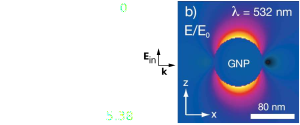
\includegraphics{abb/gmmhaertb}
\caption[GMM-FIELD, qualitative comparison with MMP results for a single particle]{
\textbf{GMM-FIELD, qualitative comparison with MMP results for a single particle.}
From the left a vertically polarised plane wave with
$\lambda = \val{532}{nm}$ 
hits a single gold particle with
$R = \val{40}{nm}$
in vacuum. The local field enhancement is shown, on the left calculated with
GMM-FIELD, on the right with MMP. MMP data are reproduced from
\cite{hae07}. The results are identical as far as this can be judged
given the different color maps. A legend for the color map is missing
from \cite{hae07}.
}\label{abb.gmmhaertb}
\end{center}
\end{figure}

We have checked whether GMM-FIELD is free of errors by trying to reproduce
the results on the field enhancement near a single gold nanoparticle that
have been obtained by H�rtling et al. with the multiple multipole method, 
MMP, \cite{hae07}.
The particle has a radius of \val{40}{nm} and is surrounded by vacuum.
It is hit by a plane wave with a wavelength of \val{532}{nm}. 
First, we will consider the field enhancement in the plane through the
center of the particle spanned by
\kvec{} and \einc{}. In \reffig{abb.gmmhaertb}, we see good qualitative
agreement between GMM-FIELD and MMP. A quantitative comparison is not
possible because the figure in \cite{hae07} has no legend for the color
scale.

\begin{figure}
\begin{center}
\includegraphics[width=\textwidth]{abb/gmmhaerta}
\caption[GMM-FIELD, quantitative comparison with MMP results for a single particle]{
\textbf{GMM-FIELD, quantitative comparison with MMP results for a single particle.}
Excitation enhancement $g_\mathrm{exc} =
|\evec \cdot \hat{\dip{}}|^2/|\einc \cdot \hat{\dip{}}|^2$ for a dipole
oriented radially (a) 
and tangentially (b) with respect to the surface of the gold nanoparticle.
Particle radius and wave lengths are the same as in
in \protect\reffig{abb.gmmhaertb}. The MMP results 
from \cite{hae07} are drawn with a red dashed line,
the results obtained with GMM-FIELD are shown as red circles.
The violet and green curves are H�rtling's results on the 
quantum efficiency and the total fluorescence enhancement and are not
of interest here (see \reffig{abb.gmmdiphaert}).
}\label{abb.gmmhaerta}
\end{center}
\end{figure}

However, the graphs on the excitation enhancement 
$\gamma_\mathrm{exc}$ in fig.~3 of
\cite{hae07} do lend themselves to a quantitative comparison of MMP and GMM-FIELD,
because the excitation enhancement is calculated as
$\gamma_\mathrm{exc} = |\evec \cdot \hat{\dip{}}|^2/|\einc \cdot \hat{\dip{}}|^2$.
We consider the two most important cases where the dipole is parallel to
the incident field \einc{}, and is oriented either radially or tangentially with respect
to the surface of the gold nanoparticle.
Both geometries and the respective results are
shown in 
\reffig{abb.gmmhaerta}. 
We see quantitative agreement. Small
deviations can be explained by differences in the dielectric function
used, the discretization error of the MMP calculation and 
numerical (i. e. rounding) errors.


% $Id: gmmdip.tex,v 1.23 2008/04/16 17:10:30 Moritz.Ringler Exp $
%
%
\section{GMM-DIP -- generalized Mie scattering of a dipole field}\label{app.gmmdip}\index{GMM-DIP}
Both GMM and GMM-FIELD use a plane wave as the incident light field. To describe
the emission of a dye molecule or an atom as in
\cite{phdrin08, rin08} the plane wave must be exchanged against that
of an oscillating dipole. The program thus obtained is called
GMM-DIP%
\footnote{The source code of GMM-FIELD  as well as some example applications
can be downloaded from
\mbox{\uri{http://moritz-ringler.name/dissertation/GMM\_DIP.tar.bz2}}.}.
GMM-DIP also differs from GMM in the output quantities:
cross sections make little sense for a dipole field and their place is taken
by the absorbed and radiated powers
$P_\mathrm{abs}/P_0$ and $P_\mathrm{r}/P_0$.

The oscillating dipole is treated like an additional particle throughout
most of the program. A 'particle index' of zero would be a canonical choice
but for practical reasons the dipole simply gets the index
$\beta = N + 1$ where $N$ is the number of scatterers.

In this fashion we arrive at the program structure for GMM-DIP that is represented
in figure~\ref{abb.gmmdip}. Changes with respect to GMM-FIELD are
highlighted in blue. The way the powers
$P_\mathrm{r}$ and $P_\mathrm{abs}$ are calculated is described in
\cite{rin08, phdrin08}. It is quite
similar to the way the cross sections are calculated in the original GMM.
In the routine that calculates the near field the initialization of
$\evec$ is changed: instead of  $\evec = \exp{i k z}\,\ex$
we now use
$\evec = \vec{0}$, the incident field is
evaluated in the same way as the scattered field of the particles.

\begin{algorithm}[ht]
\KwData{$n_\mathrm{max}$, $\lambda$, $N$; $\vec{r}^\beta$, $\vec{r}^{\mathrm{Dipol}}$, $R^\beta$, $\epsint^\beta$}
\KwResult{$g_\mathrm{r}=P_\mathrm{r}/P_0$, $g_\mathrm{ET}=P_\mathrm{abs}/P_0$}
\Begin{
read wavelength\;
read aggregate parameters\;
calculate Mie coefficients for all spheres\;
{\color{darkblue} $\beta_\mathrm{max} = N + 1$\;}
calculate vector translation coefficients\;{\color{darkblue}
\tcp{expansion of the dipole field in vector spherical harmonics}
$a^{N + 1}_{1\,1} = -i/\sqrt{3}$\;
$a^{N + 1}_{-1\,1} = i/\sqrt{3}$\;
calculate the vector translation of the dipole fields $\rightarrow p_{mn}^{0\;\beta},\ q_{mn}^{0\;\beta}$\;
$\beta_\mathrm{max} = N$\;
}
calculate scattering coefficientsn $\rightarrow a_{mn}^\beta, b_{mn}^\beta$\;
{\color{darkblue}
$\beta_\mathrm{max} = N + 1$\;
\tcp{if you want just the scattered field}
\tcp{$\beta_\mathrm{max} = N$}
}
calculate and write the near field\;
{\color{darkblue}
$\beta_\mathrm{max} = N + 1$\;
calculate $g_\mathrm{r} = P_\mathrm{r}/P_0$\;
$\beta_\mathrm{max} = N$\;
calculate $P_\mathrm{str}/P_0$\;
calculate $P_\mathrm{ext}/P_0$\;
$g_\mathrm{ET} = P_\mathrm{ext}/P_0 -  P_\mathrm{str}/P_0$\;
write $g_\mathrm{r}$ and $g_\mathrm{ET}$\;
}
}
\caption{Program structure of GMM-DIP.}\label{abb.gmmdip}
\end{algorithm}

The coordinates of the dipole that models the emitting atom or
molecule are specified in the input file defining the field and the
aggregate geometry as if it was another particle. Though the dipole
has neither radius nor refractive index both must be entered.
The value of the refractive index is not used by the program, the
'dipole radius' determines the size of the volume around the dipole
in which the field is not evaluated.

As an example, we show here the field and aggregate definition file
for a dipole that is located in the middle between two
gold particles with radius $R = \val{20}{nm}$ and
surface-to-surface distance $\dss = \val{20}{nm}$. The dipole emits at
$\lambda = \val{532}{nm}$. The whole arrangement
is immersed in water.
\begin{verbatim}
0.39886 = wavelength (vacuum wavelength: 0.532)
3 = #spheres + 1 (dipole); <= nLp in gmm01f.par
 0.03 0 0 0.02000 0.417515 1.66004 = x, y, z, r, Re(n), Im(n)
-0.03 0 0 0.02000 0.417515 1.66004 = x, y, z, r, Re(n), Im(n)
 0.00 0 0 0.00001 1.000000 0.00000 = x, y, z, (r, Re(n), Im(n)) <- dipole
\end{verbatim}
Again, we have used microns as the length unit.
The position of the dipole at the center of the coordinate system
(that is not a necessity -- it can be anywhere) is set in the last line.
The dipole orientation is always parallel to the $x$-axis, and therefore
in this case also parallel to the dimer axis. The embedding medium
is taken into account by specifying the in-water wavelength
$\lambda = \lambda_0 / \sqrt{\epsi{H2O}}$ and
by specifying the complex refractive index of the particles $\sqrt{\epsi{Au}}$
in units of the (purely real) refractive index of the medium
$\sqrt{\epsi{H2O}}$.

\subsection{Comparison with published MMP results on fluorescence
quenching near a single particle}

\begin{figure}
\begin{center}
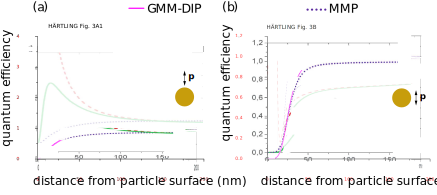
\includegraphics[width=0.8\textwidth]{abb/gmmdiphaert}
\caption[GMM-DIP, comparison with MMP results for a single particle]{
\textbf{GMM-DIP, quantitative comparison with MMP
 results for a single particle.}
 quantum efficiency for a dipole that is oriented (a) radially and (b)
 tangentially with respect to a nearby gold nanoparticle. The dipole
 has intrinsic quantum efficiency one, the particle is the same as that
in \reffig{abb.gmmhaertb}.  The MMP results from \cite{hae07}
are dotted in violet, the GMM-DIP results are shown as a magenta-colored
solid line.  The red and green lines are H�rtling's results
on the excitation enhancement and on the total enhancement and
can be ignored at this point (see also \reffig{abb.gmmhaerta}).
}\label{abb.gmmdiphaert}
\end{center}
\end{figure}

We have reproduced the MMP results on fluorescence quenching near
a single gold particle published by H�rtling et al. in \cite{hae07}
as a test of GMM-DIP. We consider the quantum efficiency of a dipole emitter
near a single gold particle with a diameter of \val{80}{nm} that emits at
$\lambda=\val{560}{nm}$ with an intrinsic quantum efficiency of one.
The surrounding medium has refractive index one. The quantum efficiency of the
quenched dipole is calculated from the Purcell factor $g_\mathrm{r}=P_\mathrm{r}/P_0$
and the energy transfer factor $g_\mathrm{ET}=P_\mathrm{abs}/P_0$ as %
\footnote{Note that the monochromatic dipole model used here is not sufficient
to describe a multi-level dye molecule. See \cite{rin08} for details.}
\begin{equation}
\eta = \frac{g_\mathrm{r}}{g_\mathrm{r} + g_\mathrm{ET}}
\end{equation}
Again we consider the two most important geometric arrangements, namely
a dipole with parallel and perpendicular orientation with respect to the
nanoparticle surface. The geometries and the results are shown in
\reffig{abb.gmmdiphaert}. GMM-DIP and MMP results agree almost perfectly.

\subsection{Feedback -
Comparison with results on fluorescence
quenching near a single particle in the Gersten-Nitzan model}
We will now compare GMM-DIP results for the Purcell factor $g_\mathrm{r}$
and the energy transfer factor $g_\mathrm{ET}$ of a dipole near a single
gold nanoparticle with the results for the same quantities
obtained with the Gersten-Nitzan model \cite{ger81}.
Apart from the fact that the Gersten-Nitzan model cannot be applied to
aggregates, it differs from GMM-DIP in two important aspects.
First, it uses a quasistatic approximation whereas GMM-DIP is fully retarded,
second, it takes into account re-excitation of the emitter by its own field
scattered by the nanoparticle. We call this phenomenon feedback.

Again, we use an example to compare the two models. We consider the
model system of \cite{dul05}: a dipole that emits at $\lambda=\val{668}{nm}$
near a nanoparticle with a diameter of \val{16}{nm} immersed in water.
Gersten-Nitzan data are calculated with ETCALC\index{ETCALC}\footnote{%
ETCALC is a C implementation of the Gersten-Nitzan model developed in our group
in Munich. The source code is available at
\mbox{\uri{http://moritz-ringler.name/dissertation/ETCALC.tar.bz2}}.
Feedback can be switched on and off by means of the compile
time parameter \texttt{GN\_FEEDBACK} in the header file
etcalc.h.}. We vary the distance between particle and dipole.
Fig.~\ref{abb.gmmdipgn} shows the Purcell
factor and the energy transfer factor for radial and tangential dipole orientation.

\begin{figure}
\begin{center}
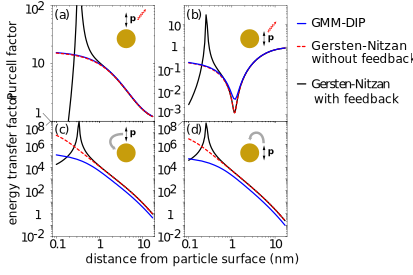
\includegraphics{abb/gmmdipgn}
\caption{
\textbf{GMM-DIP,
quantitative comparison with Gersten-Nitzan results for a single particle.}
Purcell factor (a,b) und energy transfer factor (c,d)
for a monochromatic dipole near a single gold nanoparticle; calculated with
GMM-DIP, the Gersten-Nitzan model without feedback and the
Gersten-Nitzan model with feedback.
\textbf{(a)~and (c)~radial orientation.}
\textbf{(b)~and (d)~tangential orientation.}
}\label{abb.gmmdipgn}
\end{center}
\end{figure}

Let us first have a look at the effect of feedback. This effect
becomes significant only at distances of less than \val{1}{nm} and large only at
distances of less than ca. \val{0.5}{nm}. At these distances, non-local
interactions \cite{leu90} and charge transfer \cite{dex53} cannot be neglected
any more. A distance of \val{0.5}{nm} is also comparable
to the typical size of a dye molecule. It is a rather gross approximation
to model a dye molecule with a point dipole in this situation.
Therefore, the accuracy both of the Mie-theoretical prediction and of the
Gersten-Nitzan prediction concerning the nanoparticle-induced change of the
rates is limited in this distance range. Instead, at least the molecule should
be treated quantum-mechanically. This will in general only be possible with
purely numerical methods \cite{and04}.

We now compare GMM-DIP and Gersten-Nitzan without feedback. In the
Purcell factor,
GMM-DIP and Gersten-Nitzan without feedback agree almost perfectly
(\reffig{abb.gmmdipgn}a and~b). Only the suppression of emission
for the tangential orientation at distances of about
\val{1}{nm} is more pronounced in the Gersten-Nitzan model.
The absolute difference between the GMM-DIP result and the Gersten-Nitzan
result is small and can have numerical causes or be due to small differences
in the dielectric function used.

The Gersten-Nitzan model predicts an energy transfer rate that is larger
by a factor of about two than
that predicted by the Mie-type calculation
for distances larger than about \val{1}{nm} (\reffig{abb.gmmdipgn}c and~d).
The GMM-DIP results agree with the independent MMP calculations of
\cite{hae07} as we have seen in \reffig{abb.gmmdiphaert}. Therefore, the
cause of this discrepancy is more likely to be found in the Gersten-Nitzan model
and in its implementation than in GMM-DIP.

For distances of less than about \val{0.5}{nm} the discrepancy between
Gersten-Nitzan and GMM-DIP becomes larger. This might be due to the fact that
higher order multipoles are neglected in the Gersten-Nitzan model.

In summary, we can say that the Mie-theoretical description
implemented in GMM-DIP and the Gersten-Nitzan description implemented in ETCALC
agree quantitatively in the Purcell factor and qualitatively in the energy
transfer factor if feedback is not taken into account. The effect of feedback
becomes large only at distances of less than about half a nanometer where the
assumptions underlying both models start to become less and less valid anyways.

%% $Id: pda.tex,v 1.1 2007/09/19 12:47:57 Moritz.Ringler Exp $
% Kein unabh�ngiges LaTeX-Dokument!
% Master-Dokument: diss.tex
%
% Versions-Informationen f�r diese Datei...
\RCS $Date: 2007/09/19 12:47:57 $ \RCS $Revision: 1.1 $
\RCS $Id: pda.tex,v 1.1 2007/09/19 12:47:57 Moritz.Ringler Exp $
%
\section{Das Bild-Analyse-Programm ImageJ}
\subsection{Das Particle-Analyzer-Modul}
\subsection{Das Particle-Distance-Analyzer-Modul}







%% Bibliographie
\begin{raggedright}
\bookmark[1]{\bibname}{bib}
\bibliography{bib/all-doi2url}
%\bookmark[1]{\bibliographyname}{bib}
% Bibliographie-Stil mit urlbst erzeugt aus amsplain
%\bibliographystyle{urlamsplain}
% Bibliographie-Stil erzeugt mit custom-bib und urlbst
\bibliographystyle{bst/umx}
\end{raggedright}


\end{document}
